\chapter{Prototype implementation}\label{chap:impl}

\section{Programming discipline}
The prototype was implemented largely in the spirit of exploratory programming:
``the kind where you decide what to write by writing
it.''\cite{arc}.

This approach in combination with a dynamic and flexible language like
JavaScript enables one to quickly transform ideas to working prototypes and
shape them as one goes along. But the usefulness of this method is limited, as
it may quickly produce fairly low-quality code, as it is not focused on future
maintainability.

Most of the features of the language and editor in the prototype are implemented
as a proof-of-concept, although some are more refined than others in order to
fulfil the major goals of this thesis, one of which was to implement a working
non-trivial application in the language.

\section{The language}
The prototype implementation of the language contains all the features described in Chapter \ref{chap:lang}, with the following exceptions:
\begin{itemize}
    \item Macros are not implemented.\footnote{In fact, they partially \textit{are} implemented, but are not usable. For example, there is a \texttt{macro} primitive available, which produces macro values. But it should not be used, as these macro values are not treated specially by the interpreter, so using them will not have the desired effect.}
    \item There are two primitives, which produce function values: \texttt{of} and \texttt{of-p}. The second has the same meaning as \texttt{of} described in Chapter \ref{chap:lang}. The first has the same meaning, except that it does not use pattern matching when binding names to arguments. This primitive requires that all the names must be words.
    \item Destructuring is not implemented for assignments (it does not work in \texttt{mutate}), only for definitions (it works in \texttt{bind}). Pattern matching could easily be extended to mutation, although I have found it sufficient to be usable only in definitions and ended up not implementing it for assignments in the prototype.
    \item Comments are treated as a streams of characters, taking into account nesting and balancing of brackets in multi-line comments, but are not preserved on the \acrshort{est} as a tree-like structure.
    \item Strings are not recognized specially by the parser. They are stored and manipulated as syntax tree nodes, not as streams of characters. This means that the optimization described in Section \ref{sub:str} was not applied. The performance penalty is acceptable in the prototype implementation. 
    \item The escape character \texttt{\\} has no special meaning. To substitute a special character in a string, the following built-in values are defined:
    \begin{lstlisting}
    (left-bracket) -- escapes "["
    (right-bracket) -- escapes "]"
    (left-brace) -- escapes "{"
    (right-brace) -- escapes "}"
    (pipe) -- escapes "|"
    (bang) -- escapes "!"
    \end{lstlisting}
    
    So \texttt{'[(left-bracket)hello(right-bracket)]} would evaluate to: \texttt{"[hello]"}.
\end{itemize}

Lisp's syntax is as minimal as it gets\cite{syntaxation}, which makes 

An interpreter for Lisp is also trivial to implement, so this is a good starting
point.

There are many approaches to implementing interpreters for LISP in
JavaScript\cite{js_lisps}, but the general principles are the same.

\subsection{Macros}
This
macro system is not included in the final version of the prototype, although a
proof-of-concept of it that I implemented in earlier prototypes


One feature that I experimented with while creating the prototype of Dual is
support for first-class just-in-time expanded macros

\section{The environment}

The goal is to build an online \acrlong{ide} IDE, similar to
Codeanywhere\cite{codeanywhere_website} or
Cloud9\cite{c9_website}, which works offline as well.

The current version of the development environment is intended to be used
offline, on user's machine. Nevertheless it is implemented so that it could be
easily transformed into an online system.

I decided to implement the system with minimal dependencies, so it can be easily
installed and so I can achieve a greater level of integration by having more
control over every part.

The only required dependencies for the basic functionalities of the prototype to
work is a web browser and the CodeMirror library. An additional dependency is the Node.js environment -- for running the stub of the project-manager.

The language's development environment is implemented as a web application. It
consists of three parts:
\begin{itemize}
    \item The server part, implemented in JavaScript on top of Node.js. This
      part's functions is mainly to enable access to user's file system, so any
      local folder can be opened as a project -- modern web browsers restrict
      access to the local file system, because of security reasons. The server
      part also handles persisting changes to files and configuration.
    \item The project manager part, which communicates directly with the server
      part. The connection is maintained over a
      WebSocket\cite{mdn_websockets}. This
      part provides access to user's file system via a custom folder selection
      interface. Basic configuration of server communication, such as changing
      the address and ports is also possible. Once a project is selected, the
      user may open it in the editor part.
    \item The editor part, which is the main component and can function as a
      stand-alone application. It can communicate with the server indirectly,
      through the \texttt{localStorage}
      mechanism\cite{mdn_localstorage}.
\end{itemize}

The project manager and the editor, which can be considered the front-end parts
of the system are designed to be a
\acrlong{spa}\cite{spa_wikipedia}. The
project manager exchanges JSON messages with the server through a
WebSocket. This is used for updating the view with dynamic data. In order to
facilitate the manipulation of the HTML structure of the page, which is the main
application's view, I implemented a very simple web application framework, which
binds the data from the server with the data on the client and the
\acrlong{dom}\cite[Chapter~13]{eloquentjs}.

\begin{figure}[h!]
\centering 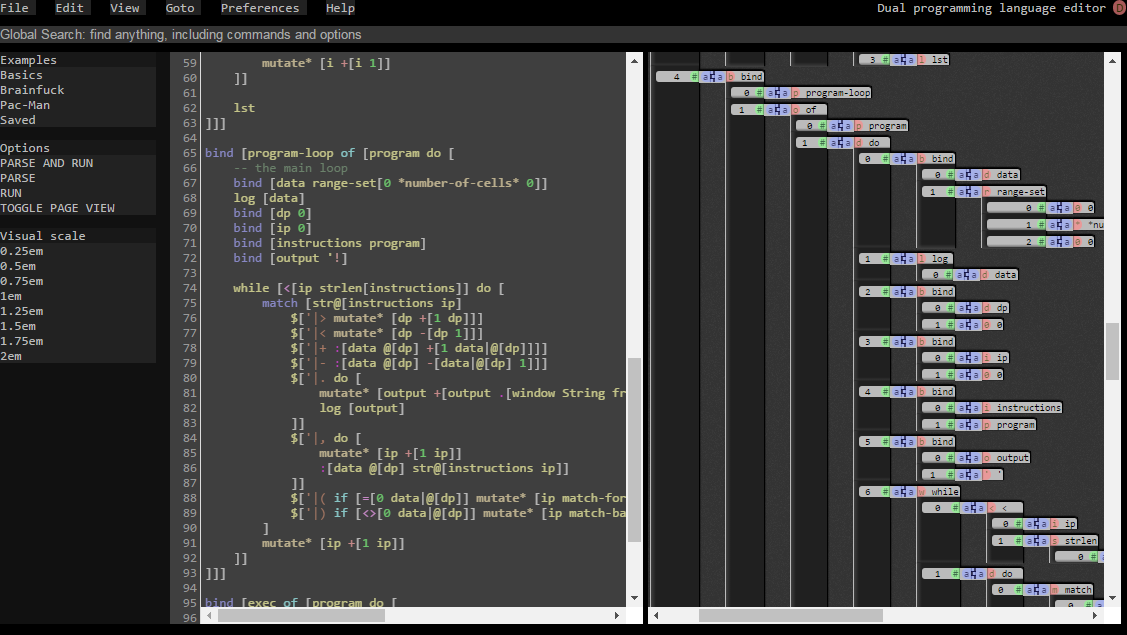
\includegraphics[width=0.9\textwidth]{editor}
\caption{The editor}
\label{fig:editor}
\end{figure}

Figure \ref{fig:editor} shows an overview of the editor prototype's window. The
basic layout is modeled after the aforementioned code editors. At the top of the
window is the menu bar, below it a mockup of a global search input (not implemented). The left panel contains basic controls for selecting examples,
invoking the parser and interpreter, toggling application view and adjusting the
scale of the visual representation.

The browser's JavaScript console is used as the standard output. There is no built-in console.

The following options are implemented in the prototype:
\begin{itemize}
    \item Available from the menu bar:
    \begin{itemize}
        \item File->Save, which saves the current content of the text editor to
          a file named \texttt{save.dual} in editor's root directory. This only
          works if the server-side part of the environment is running. Otherwise
          the source will be saved only to browser's internal storage.
        \item In the Edit menu: Undo, Redo, Cut, Copy, Paste and Select All
          options are supported. Note that by default web browsers restrict the
          access to the user's clipboard, so for Copy and Paste the standard key
          shortcuts should be used (Ctrl-C, Ctrl-V). All other conventional
          keyboard shortcuts are also supported, thanks to the CodeMirror
          library.
    \end{itemize}
    \item Available from the left panel:
    \begin{itemize}
        \item The options in the Examples submenu cause a corresponding source
          file to be loaded into the editor. This is for demonstration for the
          purposes of this thesis.
        \item The Options submenu allows the user to invoke the parser and the
          interpreter separately or in combination as well as toggling between
          the ``page'' (also known as ``application'') and visual editor
          views. The application view contains an embedded web page (iframe),
          which can be manipulated by a Dual application. This is used to
          display the game view in the Pac-Man clone example.
        \item The Visual scale submenu changes the size of the blocks in the
          visual editor. This demonstrates how manipulating one CSS property
          influences the rendering of the visual representation.
    \end{itemize}
\end{itemize}

Some options have descriptive captions available that appear when the mouse
cursor hovers over them.

\section{Text editor}
The text editor is built on top of the CodeMirror
framework\cite{codemirror_site}. It was integrated with the
editor in the following way:
\begin{itemize}
    \item A custom syntax highlighting mode for Dual was defined.  % crucial:
    \item If a position of the text cursor in or the contents of the source
      change, a fragment of text corresponding to the appropriate \acrshort{est}
      node is highlighted. Also the corresponding subtree in the visual editor
      is highlighted. This works also in the other direction -- when a node in
      the visual editor is selected, it is highlighted along with the
      corresponding text fragment. This demonstrates the core functionality of
      the system: it is ``aware'' at all times of currently focused meaningful
      part of the code, corresponding to an \acrshort{est} node. This is
      reflected in every representation that is associated with the EST.
\end{itemize}
Because every node in the EST is linked in both directions with a corresponding
abstract element in a representation, any change to the element can be reflected
in the node and, through the EST, in all other associated representations. This
makes the system accurate and fast, as every change happens in an isolated
context, which doesn't have to be reestablished every time a modification is
made.

We can distinguish three representations used by the system:
\begin{enumerate}
    \item The EST, which is the master representation of the program.
    \item The fragments of text corresponding to EST nodes in the text
      representation are tracked by CodeMirror's TextMarker objects. These
      facilitate tracking and propagating any changes to and from this
      representation, as well as highlighting.
    \item The visual representation, which is implemented in terms of pure HTML
      tables fully styled with CSS. This allows for easy and complete
      customization of the representation.
\end{enumerate}



In case of the visual representation this is implemented in a rather
straightforward way: every EST node has a corresponding set of \acrshort{dom}
nodes. Thanks to this, we can track any actions performed on the DOM through the
standard browser-implemented interface. This is solved in the prototype by
attaching \texttt{click} event handlers to relevant nodes. Such an event
triggers the following:
\begin{itemize}
    \item A corresponding EST node is ``focused'' by the system.
    \item The visual node is highlighted.
    \item A context menu appears similar to that depicted in
      \ref{fig:editor-menu}.
\end{itemize}

\begin{figure}[h!]
\centering 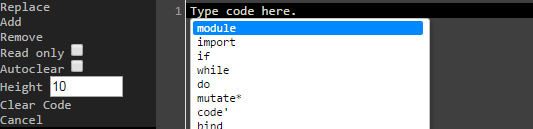
\includegraphics[width=0.9\textwidth]{editor-menu}
\caption{Visual editor's context menu}
\label{fig:editor-menu}
\end{figure}

Figure \ref{fig:editor-menu} shows the context menu that has all the basic options for manipulating the visual representation. These perform their corresponding action on the currently focused node and propagate it to the text representation. The options basic option are Replace, Add, and Remove.

The Remove option simply removes the selected node and its subtree from the
DOM, the EST, as well as the associated text fragment.

The Add and Replace options make use of the small text-editor area next to the context menu. It contains a predefined list of names of some of the possible nodes that can be inserted. Selecting any of the names causes a template for the new node -- in the form of an editable code snippet -- to be inserted into the text-editor area. Such a template can be quickly adjusted by the user before inserting.

The user may also type in raw code into the text box, without selecting any templates. After entering the code and selecting the appropriate option, the text is parsed, transformed into TextMarker, EST, and DOM representations. Then all the versions of the fragment are inserted in appropriate places.


\section{Performance}
It could be optimized similarly to CodeMirror or other web-based text editors or
applications. That is, only a visible portion (plus a margin, which allows for
fast scrolling) of the code is rendered as DOM nodes at any time. The scrollbar
is virtual and controlled by the editor rather than the browser.

Text editors like CodeMirror use similar amount of DOM nodes [[]], but thanks to
these optimizations are able to handle
megabyte-sized\cite[Section~General Approach]{cm_internals}
text files and are used in many real-world
applications\cite{cm_realworld}, which
includes being a built-in editor in developer tools in major web browsers.

Another source of inefficiency is that parsing is done twice -- once by Dual's
parser and once by CodeMirror's system, which are incompatibile.  A solution to
that would be to implement a custom text editor or extend/modify CodeMirror to
work with Dual's parser.


\begin{figure}[h!]
\centering 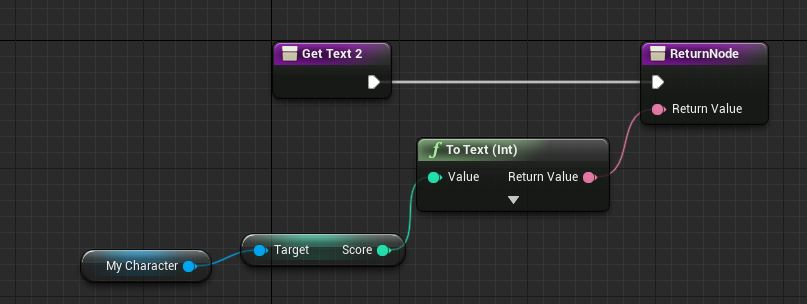
\includegraphics[width=0.9\textwidth]{blueprint}
\caption{
    Blueprints Visual Scripting;
    screenshot from \protect\cite{fig_blueprint2}
}
\label{fig:blueprint2}
\end{figure}


